\documentclass[11pt]{article}				% autres choix : book, report

\usepackage[utf8]{inputenc}					% gestion des accents (source)
\usepackage[T1]{fontenc}					% gestion des accents (PDF)
\usepackage[french]{babel}				    % gestion du français
\frenchbsetup{StandardLists=true}
\usepackage{textcomp}						% caractères additionnels
\usepackage{mathtools,amssymb,amsthm}		% packages de l'AMS + mathtools
\usepackage{lmodern}						% police de caractère
\usepackage{stmaryrd}						% symboles supplémentaires
\usepackage{csquotes}
\usepackage{empheq}							% pour encadrer.

\usepackage{geometry}						% gestion des marges
\geometry{top=1.5cm, bottom=2cm, left=2.5cm, right=2.5cm}

\usepackage{booktabs}
\usepackage{graphicx}						% gestion des images
\usepackage{xcolor}							% gestion des couleurs
\usepackage{array}							% gestion améliorée des tableaux
\usepackage{multirow}
\usepackage{multicol}						% gestion améliorée des colonnes

\usepackage[framemethod=tikz]{mdframed}		% mise en page
\usepackage{calc}							% syntaxe naturelle pour les calculs
\usepackage[pagestyles]{titlesec}			% pour les sections
\usepackage{titletoc}						% pour la table des matières
\usepackage{fancyhdr}						% pour les en-têtes
\usepackage{wrapfig}

\usepackage{tikz, pgf}
\usepackage{tikz-3dplot}
\usepackage{tkz-euclide}
\usepackage{pgfplots}						% tracer des courbes
\usepackage{pgfplotstable}

\usepackage{hyperref}						% permet de mettre des url cliquables
\usepackage{listings}						% permet de mettre du code

%\usetkzobj{all}
\usetikzlibrary{calc}
\pgfplotsset{compat=1.7}

\newcommand{\tb}{\textbackslash}
\newcommand{\cmdo}[3][]{\texttt{\textbackslash #2}\texttt{[}#1\texttt{]\{}#3\texttt{\}}}
\newcommand{\cmd}[2]{\texttt{\textbackslash #1}\texttt{\{}#2\texttt{\}}}


\title{\textbf{Guide d'utilisation de \LaTeX}
\author{Le KI'022}
\date{}
}

\setlength{\parindent}{0pt}
\begin{document}
\maketitle

\begin{figure}[h]
\begin{center}

\includegraphics[scale=0.5]{ressources/KI.png}
\end{center}
\end{figure}

\section*{Préambule}

Ce document a pour but de présenter les fonctionnalités de base et les plus utiles de LaTeX, ce langage étant devenu la norme pour produire des documents scientifiques aujourd'hui. Si vous ne connaissez absolument rien à ce langage pas de panique ! Ce guide est fait pour vous, la première section est consacrée à vous donner les bases qui vous permettrons d'écrire tous vos rapport en 1A. Ensuite, si cela vous intéresse, le guide explore plus en détails les différentes fonctionnalités offertes par LaTeX.\\

Mais d'abord je vais essayer de répondre à la question "A quoi sert {\LaTeX} ?" où plutôt, "Pourquoi me donner du mal à apprendre un langage compliqué si je peux faire plus ou moins la même chose avec Word ?". Le premier truc qu'on vous dira, c'est que LaTeX permet de faire des jolies maths, et c'est probablement ce qui vous servira le plus mais il y a d'autre manières de répondre à cette question:
\begin{itemize}
	\item LaTeX vous permets de vous concentrer uniquement sur le \textbf{contenu} de votre document et non sur la forme qui est gérée automatiquement.
	\item LaTeX demande un certain temps d'adaptation, surtout si vous êtes habitués à Word mais ensuite cela paraîtra naturel.
	\item Sans parler des maths, LaTeX procure une grande facilité pour ce qui est de référencer ses figures, ses graphiques, faire une bibliographie ou une table des matières. Il sera plus facile et surtout plus rapides de produire un rapport scientifiques avec LaTeX car tout ce que j'ai cité se fera (presque) tout seul.
\end{itemize}  

Bonne lecture !
    
\clearpage

\tableofcontents



\newpage


\section{Commencer {\LaTeX} rapidement}

\subsection{L'installation}

Avant d'écrire un document LaTeX, il vous faut une distribution de LaTeX. Le plus simple, rapide et efficace est d'utiliser le site \textit{Overleaf}. Il suffit de se connecter et de créer un nouveau document et\dots c'est tout. Il n'y a pas plus simple, le seul désavantage \footnote{Il y en a d'autres, mais peu conséquents par rapport à la facilité d'utilisation procurée par Overleaf} étant que vous allez avoir besoin d'une connexion internet, ce qui sera rarement un soucis.\\


De plus Overleaf vous permettra de travailler en simultané sur un même document, chose impossible sur un éditeur classique.

Vous trouverez quand même en annexe des conseils pour ceux qui voudraient avoir LaTeX sur leur PC.

\subsection{Les bases d'un document \LaTeX}


\noindent Pour débuter un document \LaTeX \ il faut utiliser un certain nombre de commandes et inclure des paquets\footnote{Le template fourni lors de la formation regroupe les paquets les plus utilisés en pratique.}. Voici ce à quoi chacun de vos documents devrait ressembler (commandes obligatoires en \textcolor{red}{rouge} et obligatoires pour un document en français en \textcolor{blue}{bleu}) : \\

\noindent
\textcolor{red}{\texttt{\tb documentclass[\textit{options}]\{\textit{type}\}}} \\
\textcolor{blue}{\texttt{\tb usepackage[utf8]\{inputenc\}}} \\
\textcolor{blue}{\texttt{\tb usepackage[T1]\{fontenc\}}} \\
\textcolor{blue}{\texttt{\tb usepackage[french]\{babel\}}} \\
~\\
\texttt{\tb usepackage[\textit{options}]\{\textit{nom}\}} \\
~\\ 
\texttt{\tb title\{\textit{titre}\}} \\
\texttt{\tb author\{\textit{auteur}\}} \\
\texttt{\tb date\{\textit{date}\}} \\
~\\ 
\textcolor{red}{\texttt{\tb begin\{document\}}}\\
\texttt{\tb maketitle} \\
\texttt{\tb taleofcontents} \\
~\\
\texttt{\tb section\{\textit{Titre de la section}\}} \quad (\texttt{\tb section*} pour éviter la numérotation)	 \\
\texttt{\tb subsection\{\textit{Titre de la sous-section}\}} \\
\textit{Votre texte}\\

\texttt{\tb subsection\{\textit{Titre de la sous-section}\}} \\
\textit{Votre texte} \\
~\\
\textcolor{red}{\texttt{\tb end\{document\}}} \\

Vous pouvez déjà essayer de reproduire ce schéma (sans le \texttt{\tb usepackage} en noir pour le moment) avec \texttt{\tb documentclass[11pt]\{article\}},remplacez juste ce qui est en italique par le titre, auteur, date, etc\dots et vous devriez avoir un document qui ressemble à ceci:
\clearpage
\begin{figure}
\begin{center}
	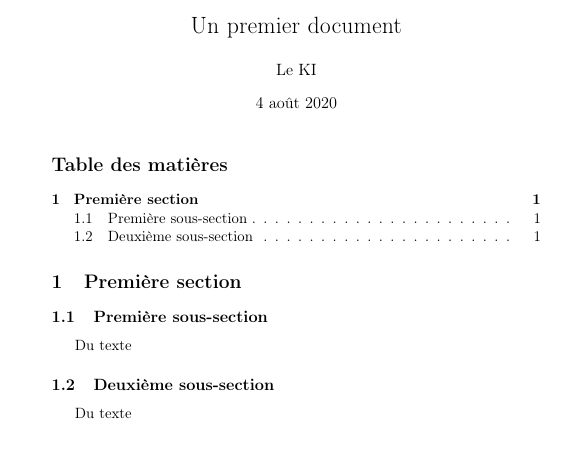
\includegraphics[scale=0.5]{ressources/frover.png}
\end{center}	

\end{figure}



Pas mal non ? En quelques lignes vous avez déjà un document prêt à être rendu.

\subsection{Les commandes classiques de mise en page}


\noindent Pour modifier le texte, il y a les commandes : \\
\begin{multicols}{2}


\begin{tabular}{lclc}
Commande &  & Rendu & Raccourci \\
\verb?\textbf{?\emph{texte}\verb?}? & $\rightarrow$ & \textbf{texte} & Ctrl + B \\
\verb?\textit{?\emph{texte}\verb?}? & $\rightarrow$ & \textit{texte} & Ctrl + I \\
\verb?\texttt{?\emph{texte}\verb?}? & $\rightarrow$ & \texttt{texte} & \\
\verb?\underline{?\emph{texte}\verb?}? & $\rightarrow$ & \underline{texte}  & \\
\verb?\emph{?\emph{texte}\verb?}? & $\rightarrow$ & \emph{texte} & \\
\verb?\textsc{?\emph{texte}\verb?}? & $\rightarrow$ & \textsc{texte} &  \\
\verb?\fbox{?\emph{texte}\verb?}? & $\rightarrow$ & \fbox{texte} & \\

\end{tabular}\\

\columnbreak

Selon les éditeurs (Overleaf ou autre), il peut y avoir plusieurs raccourcis que ceux-ci, néanmoins il est toujours possible de les utiliser façon "Word", c'est à dire sélectionner le texte à mettre en italique par exemple puis d'appuyer sur Ctrl+I.

\end{multicols}

\begin{multicols}{2}


\noindent Les listes à puces (respectivement numérotées) se font avec les commandes suivantes : \\

\begin{tabular}{lcl}

\verb?\begin{itemize}? & ou & \verb?\begin{enumerate}? \\
\indent \verb?\item? \emph{texte} &  & \indent \verb?\item? \emph{texte} \\
\indent \verb?\item? \emph{texte} &  & \indent \verb?\item? \emph{texte} \\
\verb?\end{itemize}? &  & \verb?\end{enumerate}? \\

\end{tabular} \\

\columnbreak

Pour des listes avec des $\bullet$ plutôt que des tirets, mettre la commande \texttt{\tb frenchbsetup\{StandardLists=true\}} en début de document (avant le \texttt{\tb begin\{document\}}). On peut également "empiler" plusieurs listes en cascade, elles seront indentées au fur et à mesure.
\end{multicols}

$\rightarrow$ En LaTeX, le \texttt{\tb begin\{\}} suivi d'un \texttt{\tb end\{\}} s'appelle un environnement, cela permet de formater ce que vous allez mettre entre ces deux commandes. \textcolor{red}{Faire attention à bien mettre le \texttt{\tb begin} et le \texttt{\tb end} sinon ça ne marchera pas !} \\
\clearpage
\textbf{Pour les sauts de lignes et paragraphes :} \\

Vous l'avez peut-être remarqué mais en LaTeX, pour revenir a la ligne vous pouvez pas juste appuyer sur la touche \texttt{Enter}, il vous faut soit laisser une ligne blanche, mettre un double backslash \texttt{\tb \tb} à la fin de votre ligne (les deux combinés donne un saut de ligne) ou utiliser la commande \texttt{\tb newline}.
En fait le retour à la ligne vous permettra de faire un nouveau paragraphe, celui-ci sera indenté par défaut (décalé vers la droite) pour palier ce problème il suffit de mettre \texttt{\tb noindent} en début de ligne ou, pour le faire pour tout le document, mettre la commande \texttt{\tb setlength\{\tb parindent\}\{0pt\}} en début de document (avant le \texttt{\tb begin\{document\}}).\\
Pareillement, les espaces ne se font pas en appuyant 40 fois sur la touche espace, il faut utiliser des commandes telles que \texttt{\tb quad} et \texttt{\tb qquad}.

\begin{multicols}{2}


\noindent Les citations se font de la façon suivante : \\
\verb?\begin{quote}? \\
\emph{texte} \\
\verb?\end{quote}? \\

\noindent Et pour des citations de plusieurs lignes : \\
\verb?\begin{quotation}? \\
\emph{texte} \\
\verb?\end{quotation}? 

\columnbreak

\noindent La commande \verb?\footnote{?\emph{texte}\verb?}? crée une note en bas de page. \\


\noindent La position du texte sur la page se modifie avec les environnements \texttt{ flushleft, center,  flushright}. C'est certainement le 2e qui vous sera le plus utile: \\
\verb?\begin{center}? \\
\emph{texte}\\
\verb?\end{center}? 

\end{multicols}

Voila pour le texte pur et simple, j'en profite pour dire qu'il ne faut pas mémoriser toutes les commandes, par exemple pour les listes, il existe plein d'options pour modifier le type de liste ou même en faire plusieurs en cascade etc\dots Mais il est inutile de retenir tout cela, une simple recherche sur internet vous donnera ce que vous voulez savoir ! Vous trouverez aussi dans ce guide une description des options les plus utiles dans la section [Section name].

\subsection{Les images, tableaux et autres flottants}

Un des points les plus importants dans un document est l'inclusion d'images, leur référencement et les disposer intelligemment pour ne pas perturber la lecture. Sur ce point, il peut être très compliqué de vouloir faire exactement ce que l'on a en tête en LaTeX car contrairement aux logiciels Office, on ne peut pas déplacer l'image avec la souris.
Pas exactement certes mais pour la plupart de vos documents, LaTeX va gérer très bien tout seul votre placement d'images.\\

Commençons pas le plus basique, le \cmdo[scale=\textit{échelle}]{includegraphics}{\textit{chemin d'accès à l'image}}.Disons que vous ayez une image \texttt{image.png} dans le même dossier que votre fichier .tex (sur Overleaf vous pouvez directement importer vos images). Pour mettre cette image dans votre document il y a juste besoin d'écrire deux choses: \\

\begin{itemize}
	\item \cmd{usepackage}{graphicx} en début de document.
	\item \cmdo[scale=$x$]{includegraphics}{image.png} \quad ()avec $x$ le facteur d'échelle entre 0 et 1) là où vous voulez insérer votre image.
\end{itemize}
\clearpage

Bien sur cette commande fonctionne dans les environnements cités ci-dessus, par exemple si vous voulez centrer votre image: \\


\begin{multicols}{2}
\cmd{begin}{center}\\
\cmdo[scale=$x$]{includegraphics}{image.png} \\
\cmd{end}{center}\\

\columnbreak

D'autres paramètres sont possibles plutôt que le scale, voir section [Section name]
\end{multicols}


\textbf{Les flottants}\\

La méthode présentée ci-dessus permet de dire à LaTeX précisément où doivent être insérées vos images. Mais il peut être parfois plus judicieux de laisser LaTeX organiser vos images, pour cela on utilise des flottants (non ce n'est pas pareil que des flottants en info...). Les flottants tiennent leur nom du fait que LaTeX va les déplacer à sa convenance pour faire le meilleur document possible (selon lui libre à vous de changer ensuite).\\

Prenons l'exemple de l'image précédente, nous allons maintenat la mettre dans un environnement supplémentaire nommé \texttt{figure}: \\

\begin{multicols}{2}
\cmd{begin}{figure}\texttt{[}h\texttt{]}\\
\texttt{\tb centering} \quad (Equivalent à un center)
\cmdo[scale=$x$]{includegraphics}{image.png} \\
\cmd{caption}{légende}\\
\cmd{end}{figure}\\
Sans le \texttt{\tb centering}, l'image sera à gauche. 

\columnbreak

L'argument "h" indique que l'on veut que notre image soit ici ("here"), c'est à dire là où on écrit le texte. On peut aussi mettre b ou t pour "top" et "bottom" par exemple, ainsi notre image se retrouvera en haut ou en bas de la page peut importe où l'on a écrit la commande.
\end{multicols}


\begin{figure}[h!]
	\centering
	
\includegraphics[scale=0.2]{ressources/KI.png}
	\caption{Le logo du KI}
\end{figure}



Voici une image incorporée dans un document avec les commandes ci-dessus. Il y a plein de manière de modifier la légende et l'image à votre convenance, comme l'encadrer, l'inclure dans du texte(package \texttt{wrapfig}) et d'autres. Plus de détails sont donnés dans la section [section name].\\


$\rightarrow$ Attention cependant, LaTeX peut décider de ne pas respecter votre argument entre crochet \texttt{[]} si cela conduit l'image à déborder de la page ou à trop éloigner le titre d'une section de son texte.\\

Un autre exemple de flottants : Les tableaux, ceux-ci ont une syntaxe bien précise mais il existe certains sites comme tablesgenerator.com qui vous simplifie la vie, vous avez juste à rentrer vos donnés et il vous génère le code automatiquement.

\clearpage

\subsection{Ecrire des mathématiques}

On aborde ici une grosse partie de ce que vous allez faire en LaTeX, au début cela va être un peu laborieux, car vous passerez votre temps à regarder la magnifique fiche mémo faite par le KI (disponible à l'adresse latex.enpc.org) avec entre autre les commandes mathématiques. Mais ces commandes sont assez naturels et vous les mémoriserez assez vite.\\

Avant toute chose, assurez vous d'avoir mis \cmd{usepackage}{amsmath} en préambule.

Pour écrire des maths, c'est très simple, il suffit de se placer dans un environnement mathématique, obtenu avec \texttt{\tb( \tb)} ou \texttt{\tb[ \tb]}. 

\begin{multicols}{2}
Ainsi le code suivant:\\
\textsf{Le théorème de Pythagore \texttt{\tb(} $\text{x}^{\wedge}$2+ $\text{y}^{\wedge}$2 = $\text{z}^{\wedge}$2 \texttt{\tb)} a été prouvé faux pour des puissances supérieures. Cela veut dire que l'équation suivante n'a pas de solutions entières:
	 \texttt{\tb[} $\text{x}^{\wedge}$n + $\text{y}^{\wedge}$n = $\text{z}^{\wedge}$n \texttt{\tb}] }
	
	\columnbreak
	
	Devient sur le pdf:\\	
	Le théorème de Pythagore $x^2 + y^2 = z^2$ a été prouvé faux pour des puissances supérieures. Cela veut dire que l'équation suivante n'a pas de solutions entières: \[ x^n + y^n = z^n \]
	
	
	
\end{multicols}
Observez la différences entre les deux, le \texttt{\tb( \tb)} permet d'écrire des maths sur la même ligne que le texte en cours alors que \texttt{\tb[ \tb]} centre vos maths en sautant une ligne (\textbf{inline} vs \textbf{display} mode). Vous pouvez aussi utiliser le \$ plutôt \texttt{\tb(} et \texttt{\tb)} pour un environnement inline.

Si vous voulez numéroter vos équations alors il faut utiliser l'environnement \texttt{equation}:
\begin{equation}
x^2 +y^2 = z^2
\end{equation}

Vous pouvez inclure toutes sortes de symboles dans un environnement mathématiques comme des lettres grecques $\alpha \ \beta \ \gamma$, des signes logiques et quantificateurs $\forall \ \exists \bigcup \sum$. La plupart de ces symboles sont répertoriés dans la fiche mémo distribuée lors de la formation ou disponible latex.enpc.org.\\

\textbf{Puissance et indice}\\

Pour écrire des puissances et des indices à coté d'une variable ou d'un symbole, il faut utiliser \verb|^ et _|.

\begin{multicols}{2}
Le code suivant:\\

\verb|\[ a_1^2 + a_2^2 = a_3^2 \]| \\

En utilisant des \texttt{\{ \}} lorsque les exposants/indices ne sont pas un seul symbole:\\

\verb|\[ x^2{2 \alpha} - 1 = y_{ij} + y_{ij} \]|\\

Plus compliqué:\\

\verb|\[ \sum_{i=1}^{\infty} \frac{1}{n^s} =| \\
\verb| \prod_p \frac{1}{1 - p^{-s}} \] |

\columnbreak

Devient sur le pdf:\\

$$ a_1^2 + a_2^2 = a_3^2$$\\
$$ x^2{2 \alpha} - 1 = y_{ij} + y_{ij} $$\\
\[ \sum_{i=1}^{\infty} \frac{1}{n^s} = \prod_p \frac{1}{1 - p^{-s}} \]

\end{multicols}



\newpage



\subsection{Complément}


\subsubsection{Inclure du code}


\noindent Il est également possible d'inclure du code dans un fichier \LaTeX \ grâce au paquet \verb?\usepackage{listings}? et aux commandes suivantes : \\

\noindent \verb?\lstset{language=? \emph{nom de langage} \verb?}? \\
\verb?\begin{lstlisting}? \\
\emph{Le code, tel qu'il serait écrit dans un éditeur de texte classique. Exemple de code Python :} \\
for i in range (0: N) : \\
\indent X[i] = methode(X[i - 1]) \\
\verb?\end{lstlisting}? \\

\noindent Cela va inclure le code ainsi :

\lstset{language=c++}
\begin{lstlisting}

// New function.
int function(int x) {
    return x * 10;
}

for (int i = 0; i < 10; i++) {
	int j = function(i);
	std::cout << j << std::endl;
}

\end{lstlisting}

\noindent Il existe de nombreuses options pour ajouter la coloration syntaxique, encadrer le code, numéroter les lignes, mais les liens fournis en \ref{lien} expliquent tous ces détails.


\subsubsection{Liens utiles}\label{lien}


\noindent Voici quelque lien utile pour chercher des commandes, des options ou des précisions supplémentaires :
\begin{itemize}
	\item \url{https://www.google.com}
	\item \url{tex.stackexchange.com}
	\item \url{https://fr.wikibooks.org/wiki/LaTeX}
	\item \url{https://openclassrooms.com/courses/redigez-des-documents-de-qualite-avec-latex}
	\item \url{https://fr.sharelatex.com}
	\item \url{https://upont.enpc.fr/ponthub/autres}
\end{itemize}


\subsubsection{Logiciel conseillé}


\noindent ShareLaTeX est une solution pratique pour s'éviter l'installation de \LaTeX \ et faire des projets à plusieurs\footnote{Deux maximum sur la version gratuite.}, néanmoins, il peut être utile d'avoir \LaTeX \ sur son propre ordinateur et donc d'avoir un logiciel de traitement de texte adapté : Sublime Text \footnote{Sublime Text doit être configuré pour gérer \LaTeX.} et TexMaker sont de bons logiciel testés et approuvés par le KI'018.

\section{Formatage de texte}

\section{Design de pages}

\section{Les listes}

\section{Tableaux et images}

\section{Références}

\section{Maths avancées}

\section{Choisir sa police}

\section{Pour aller plus loin}

\section{Les erreurs les plus communes}

\end{document}